\vfill
\setlength{\fboxsep}{4.5pt}
\noindent\fcolorbox{gray}{white}{\parbox{\fboxwidth}{%
	\begin{wrapfigure}{r}{0.3\textwidth}
		\vspace{-1em}
		\centering 
		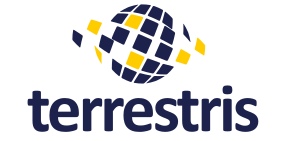
\includegraphics[width=\linewidth]{105_terrestris}
		\vspace{-1em}
	\end{wrapfigure}	
	\textbf{Silbersponsor}\\	
	\noindent terrestris bietet Dienstleistungen und Produkte mit Open-Source-Software an und 
	ist dabei insbesondere auf Geodateninfrastrukturen, webbasierte Informationssysteme und WebMapping-Anwendungen fokussiert, 
	die neben 2D- auch 3D-Daten enthalten und auch für mobile Endgeräte optimiert sind.
	%
	Wir orientieren uns dabei an den Anforderungen unserer Kunden und realisieren auf 
	den jeweiligen Bedarf zugeschnittene Lösungen.
	Neben der Anwendungsentwicklung können unsere Kunden Support und Schulungen für 
	verschiedene Open-Source-Softwaretools, z.\,B. PostgreSQL/PostGIS, UMN Mapserver, 
	GeoServer, SHOGun, OpenLayers, GeoExt, ExtJS und QGIS, erhalten.
	%
	National und international gut vernetzt bieten wir zusammen mit unseren Partnerfirmen
	Wartung und Support zu Open-Source-Produkten/Projekten wie SHOGun, GeoServer oder OpenLayers an.
	Diese Rahmenbedingungen erlauben uns unvoreingenommen Lösungen zu entwickeln und 
	anzubieten, die tatsächlich alle Anforderungen unserer Kunden zufrieden stellen.
	}
}
\setlength{\fboxsep}{3pt}
\vfill